\documentclass[11pt,a4paper]{article}

% ------------------------------------------------------------------ pacotes
\usepackage[utf8]{inputenc}
\usepackage[T1]{fontenc}
\usepackage{lmodern}
\usepackage{microtype}
\usepackage[a4paper,margin=2.5cm]{geometry}
\usepackage{graphicx}
\usepackage{float}
\usepackage{booktabs}
\usepackage{tabularx}
\usepackage{array}
\usepackage{xcolor}
\usepackage{enumitem}
\usepackage{caption}
\usepackage{fancyhdr}
\usepackage{listings}
\usepackage{tikz}
\usetikzlibrary{positioning,arrows.meta,shapes.geometric,fit,backgrounds}
\usepackage[hidelinks]{hyperref}

% ------------------------------------------------------------------ português (sem babel)
\renewcommand{\figurename}{Figura}
\renewcommand{\tablename}{Tabela}
\renewcommand{\contentsname}{Sumário}
\renewcommand{\refname}{Referências}
\renewcommand{\lstlistingname}{Listagem}
\hyphenpenalty=2000
\tolerance=1000
\emergencystretch=2em

% ------------------------------------------------------------------ dados da dupla
\newcommand{\alunoA}{Lara Strutz Carvalho -- 2023039325}
\newcommand{\alunoB}{Rian Rero Lopes Jericó Vieira -- 2023039473}
\newcommand{\linkvideo}{[LINK DO VÍDEO]}

% ------------------------------------------------------------------ estilo
\definecolor{azul}{HTML}{1F3A5F}
\definecolor{cinza}{HTML}{F4F6F8}
\definecolor{verde}{HTML}{2E7D32}
\definecolor{vermelho}{HTML}{C62828}
\captionsetup{font=small,labelfont=bf}
\newcolumntype{L}{>{\raggedright\arraybackslash}X}
\setlist{itemsep=2pt,topsep=4pt}
\setlength{\parskip}{4pt}

\lstset{
  basicstyle=\ttfamily\footnotesize,
  backgroundcolor=\color{cinza},
  frame=single, rulecolor=\color{black!20},
  breaklines=true, columns=fullflexible, keepspaces=true,
  showstringspaces=false, xleftmargin=4pt, xrightmargin=4pt,
  literate={á}{{\'a}}1 {é}{{\'e}}1 {í}{{\'i}}1 {ó}{{\'o}}1 {ú}{{\'u}}1
           {â}{{\^a}}1 {ê}{{\^e}}1 {ô}{{\^o}}1 {ã}{{\~a}}1 {õ}{{\~o}}1
           {ç}{{\c{c}}}1 {Ç}{{\c{C}}}1 {Ã}{{\~A}}1 {É}{{\'E}}1 {°}{{\textdegree}}1
}

\pagestyle{fancy}
\fancyhf{}
\fancyhead[L]{\small TP Final -- SDA}
\fancyhead[R]{\small OPC UA, Node-RED e MQTT}
\fancyfoot[C]{\thepage}
\renewcommand{\headrulewidth}{0.4pt}

\begin{document}

% ================================================================== capa
\begin{titlepage}
  \centering
  {\large Universidade Federal de Minas Gerais\\
  Escola de Engenharia\\
  Departamento de Engenharia Eletrônica\par}
  \vspace{0.6cm}
  {\large Sistemas Distribuídos para Automação\par}
  \vfill
  {\color{azul}\rule{\linewidth}{1pt}\par}
  \vspace{0.4cm}
  {\LARGE\bfseries Trabalho Prático Final\par}
  \vspace{0.3cm}
  {\Large Integração de Sistemas Industriais utilizando\\ OPC UA, Node-RED e MQTT\par}
  \vspace{0.3cm}
  {\large Supervisão de um tanque de armazenamento com bomba de transferência\par}
  \vspace{0.4cm}
  {\color{azul}\rule{\linewidth}{1pt}\par}
  \vfill
  {\large \alunoA\\ \alunoB\par}
  \vspace{0.8cm}
  {\large Professor: Armando Alves Neto\par}
  \vspace{0.4cm}
  {Vídeo de demonstração: \linkvideo\par}
  \vfill
  {\large Belo Horizonte, novembro de 2026\par}
\end{titlepage}

\tableofcontents
\newpage

% ================================================================== 1
\section{Introdução}

Em uma planta industrial, os equipamentos disponibilizam um grande número de
variáveis, mas o valor instantâneo dessas variáveis não basta: é preciso
acompanhar a sua evolução, detectar situações anormais e entregar essas
informações a outras aplicações. Este trabalho implementa uma arquitetura
simplificada de \emph{Industrial Internet of Things} (IIoT) para resolver esse
problema, usando três tecnologias em níveis diferentes do sistema:

\begin{itemize}
  \item \textbf{OPC UA}, para acessar de forma estruturada as variáveis do
        processo, disponibilizadas pelo \emph{Prosys OPC UA Simulation Server};
  \item \textbf{Node-RED}, como cliente OPC UA, elemento de processamento e
        \emph{dashboard} de supervisão;
  \item \textbf{MQTT}, com o broker \emph{Eclipse Mosquitto}, para distribuir as
        informações a outras aplicações segundo o modelo
        \emph{publish/subscribe}.
\end{itemize}

Todos os componentes foram executados em um único computador com Linux. O
processo escolhido foi um \textbf{tanque de armazenamento com uma bomba de
transferência}.

% ================================================================== 2
\section{Processo escolhido}

O processo representa um tanque de armazenamento de água (\texttt{Tanque01}) do
qual uma bomba (\texttt{Bomba01}) retira o líquido e o envia para a linha de
produção. As grandezas monitoradas são:

\begin{itemize}
  \item \textbf{nível do tanque} (\%), medido continuamente;
  \item \textbf{temperatura do líquido} no tanque (°C);
  \item \textbf{vazão de saída da bomba} (L/min);
  \item \textbf{estado da bomba} (ligada/desligada), que também pode ser
        comandado pelo operador;
  \item \textbf{limite de nível alto} (\%), parâmetro de alarme ajustável pelo
        operador e armazenado no próprio servidor OPC UA.
\end{itemize}

Esse processo foi escolhido por ser simples e por permitir condições anormais
fáceis de entender, como a bomba ligada sem vazão (possível falha de
bombeamento), o nível fora da faixa e a temperatura elevada.

% ================================================================== 3
\section{Arquitetura do sistema}

A Figura~\ref{fig:arquitetura} mostra a arquitetura implementada. O servidor
OPC UA faz o papel do ``equipamento''. O Node-RED lê as variáveis via OPC UA,
processa os dados, alimenta o \emph{dashboard} e publica as informações no
broker MQTT. Qualquer cliente que assine os tópicos recebe as mensagens, sem
que o Node-RED precise conhecê-lo.

\begin{figure}[H]
\centering
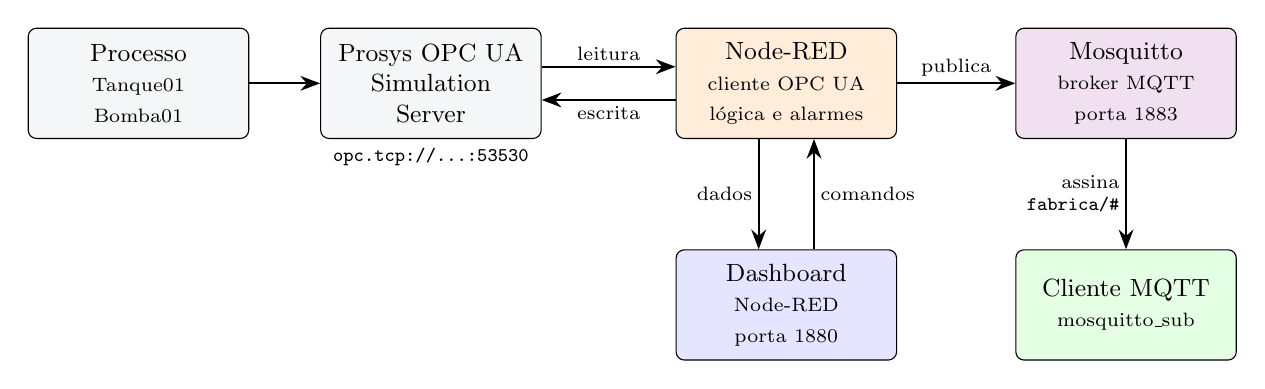
\begin{tikzpicture}[
  bloco/.style={draw, rounded corners=3pt, fill=cinza, align=center,
                minimum width=2.8cm, minimum height=1.4cm, font=\small},
  seta/.style={-{Stealth[length=2.5mm]}, thick},
  rot/.style={font=\scriptsize, inner sep=2pt}
]
  \node[bloco] (proc) {Processo\\\scriptsize Tanque01\\\scriptsize Bomba01};
  \node[bloco, right=0.9cm of proc] (opc) {Prosys OPC UA\\Simulation\\Server};
  \node[bloco, right=1.7cm of opc, fill=orange!15] (nr) {Node-RED\\\scriptsize cliente OPC UA\\\scriptsize lógica e alarmes};
  \node[bloco, right=1.5cm of nr, fill=violet!12] (broker) {Mosquitto\\\scriptsize broker MQTT\\\scriptsize porta 1883};
  \node[bloco, below=1.4cm of nr, fill=blue!10] (dash) {Dashboard\\\scriptsize Node-RED\\\scriptsize porta 1880};
  \node[bloco, below=1.4cm of broker, fill=green!10] (sub) {Cliente MQTT\\\scriptsize mosquitto\_sub};

  \draw[seta] (proc) -- (opc);
  \draw[seta] ([yshift=6pt]opc.east) -- node[rot, above] {leitura} ([yshift=6pt]nr.west);
  \draw[seta] ([yshift=-6pt]nr.west) -- node[rot, below] {escrita} ([yshift=-6pt]opc.east);
  \draw[seta] ([xshift=-10pt]nr.south) -- node[rot, left] {dados} ([xshift=-10pt]dash.north);
  \draw[seta] ([xshift=10pt]dash.north) -- node[rot, right] {comandos} ([xshift=10pt]nr.south);
  \draw[seta] (nr) -- node[rot, above] {publica} (broker);
  \draw[seta] (broker) -- node[rot, left, align=right] {assina\\\texttt{fabrica/\#}} (sub);
  \node[rot, below=1pt of opc, align=center] {\texttt{opc.tcp://...:53530}};
\end{tikzpicture}
\caption{Arquitetura implementada.}
\label{fig:arquitetura}
\end{figure}

A Tabela~\ref{tab:componentes} resume o papel de cada componente e as versões
utilizadas.

\begin{table}[H]
\centering
\small
\caption{Componentes do sistema.}
\label{tab:componentes}
\begin{tabularx}{\linewidth}{@{}l l L@{}}
\toprule
\textbf{Componente} & \textbf{Versão} & \textbf{Papel} \\
\midrule
Prosys OPC UA Simulation Server & 2026.2.2 & Servidor OPC UA que expõe as variáveis do processo \\
Node.js & 26.5.0 & Ambiente de execução do Node-RED \\
Node-RED & 5.0.9 & Integração, processamento e supervisão \\
node-red-contrib-opcua & 0.2.355 & Nós de cliente OPC UA (leitura e escrita) \\
@flowfuse/node-red-dashboard & 1.37.0 & \emph{Dashboard} 2.0 do Node-RED \\
Eclipse Mosquitto & 2.1.2 & Broker MQTT (contêiner Docker \texttt{eclipse-mosquitto:2}) \\
mosquitto\_sub & 2.1.2 & Cliente MQTT adicional (assinante) \\
\bottomrule
\end{tabularx}
\end{table}

% ================================================================== 4
\section{Variáveis OPC UA}

\subsection{Endpoint}

O Node-RED se conecta ao servidor pelo endpoint
\begin{center}
\texttt{opc.tcp://localhost:53530/OPCUA/SimulationServer}
\end{center}
com política de segurança \emph{None} e usuário anônimo, o que é adequado para
um ambiente local de testes. Em uma instalação real seriam usados os modos
\emph{Sign} ou \emph{SignAndEncrypt}, com certificados e autenticação de
usuário.

\subsection{Address Space}

No Prosys foi criado, dentro de \texttt{Objects}, o objeto \texttt{Processo},
com uma pasta para cada equipamento (Figura~\ref{fig:prosys}). As variáveis,
seus tipos e os NodeIds usados estão na Tabela~\ref{tab:variaveis}. Foram
usados os três tipos de dado (\emph{Float}, \emph{Int32} e \emph{Boolean}) e
variáveis somente de leitura e de leitura/escrita.

\begin{table}[H]
\centering
\small
\caption{Variáveis OPC UA utilizadas (acesso: L = somente leitura; L/E = leitura e escrita).}
\label{tab:variaveis}
\begin{tabularx}{\linewidth}{@{}l >{\footnotesize}l l l L@{}}
\toprule
\textbf{Variável} & \textbf{NodeId} & \textbf{Tipo} & \textbf{Acesso} & \textbf{Significado} \\
\midrule
Nivel           & \texttt{ns=3;i=1010}           & Float   & L & Nível do tanque, em \% da altura útil \\
Temperatura     & \texttt{ns=3;i=1011}     & Float   & L & Temperatura do líquido no tanque (°C) \\
LimiteNivelAlto & \texttt{ns=3;i=1012} & Int32   & L/E & Limite de alarme de nível alto (\%), ajustado pelo operador \\
Ligada          & \texttt{ns=3;i=1014}           & Boolean & L/E & Estado/comando da bomba (\texttt{true} = ligada) \\
Vazao           & \texttt{ns=3;i=1015}            & Float   & L & Vazão de saída da bomba (L/min) \\
\bottomrule
\end{tabularx}
\end{table}

O comportamento de cada variável foi configurado na aba \emph{Value} do Prosys
(campo \emph{Value Type} e parâmetros \emph{Min Value}, \emph{Max Value},
\emph{Period} e \emph{Initial Value}). O nível segue um sinal senoidal entre 40 e
80\% com período de 120~s. A temperatura varia aleatoriamente entre 28 e 34~°C
e a vazão, entre 12 e 16~L/min. A bomba (\texttt{Ligada}) e o limite de nível alto
são valores constantes, inicialmente \texttt{true} e 90\%, alterados pelo
\emph{dashboard}. O projeto do Prosys foi salvo no arquivo
\texttt{project.uasim}, entregue junto com o trabalho.

\begin{figure}[H]
\centering
\IfFileExists{figuras/prosys_address_space.png}{%
  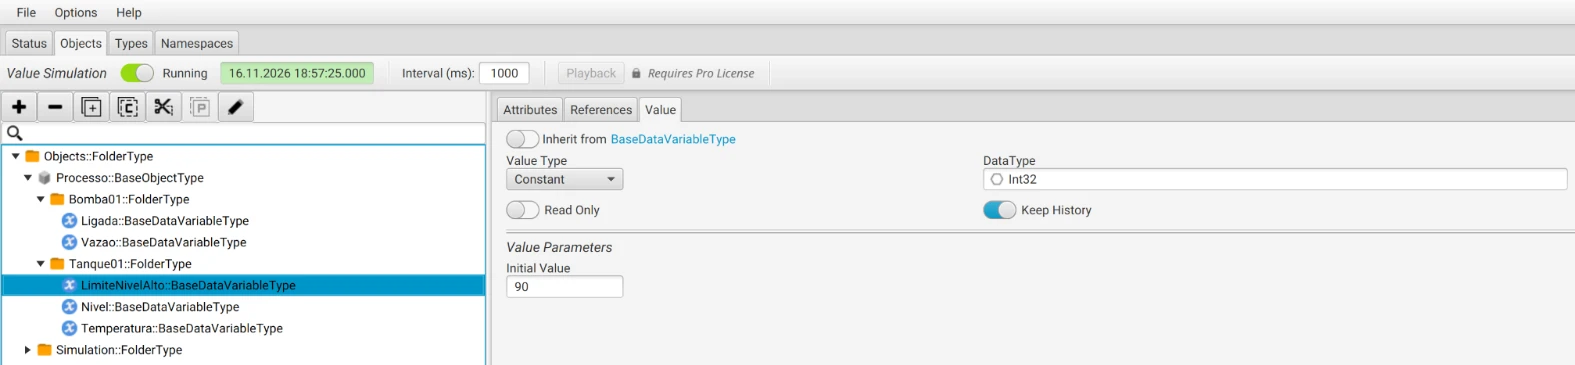
\includegraphics[width=\linewidth]{figuras/prosys_address_space.png}%
}{%
  \fbox{\parbox[c][4cm][c]{0.8\linewidth}{\centering\color{vermelho}\bfseries
  INSERIR AQUI O PRINT DO ADDRESS SPACE NO PROSYS\\
  (salvar como relatorio/figuras/prosys\_address\_space.png)}}%
}
\caption{Address Space criado no Prosys OPC UA Simulation Server (aba \emph{Objects}). À direita, a aba \emph{Value} da variável \texttt{LimiteNivelAlto}: tipo Int32, valor constante 90 e \emph{Read Only} desligado (leitura/escrita).}
\label{fig:prosys}
\end{figure}

\subsection{Aquisição no Node-RED}

A aquisição está na aba \emph{1 -- Aquisição OPC UA e Lógica}
(Figura~\ref{fig:fluxo1}) e segue estes passos:

\begin{enumerate}
  \item Ao iniciar o fluxo, o nó \emph{Configuração dos NodeIds} grava no
        contexto global a lista de variáveis, com NodeId e tipo de cada uma.
        Os NodeIds ficam centralizados nesse único nó.
  \item Um nó \emph{inject} dispara a cada 1~s. O nó \emph{Gerar pedidos de
        leitura} cria uma mensagem por variável, com
        \texttt{msg.topic} igual ao NodeId.
  \item O nó \emph{OPC UA Client} (ação \texttt{read}) executa a leitura de
        cada NodeId (serviço \emph{Read}, atributo \emph{Value}) e devolve o
        valor em \texttt{msg.payload}.
  \item Um nó \emph{change} troca o tópico pelo nome da variável e um nó
        \emph{join} junta as cinco leituras em um único objeto, por exemplo
        \texttt{\{nivel, temperatura, vazao, bombaLigada, limiteNivelAlto\}}.
  \item O objeto segue para a lógica do processo.
\end{enumerate}

Foi usada leitura cíclica (\emph{polling}) de 1~s porque o processo é lento em
relação a esse período e porque assim todas as variáveis chegam juntas a cada
ciclo, o que simplifica a lógica que as combina. Erros do cliente OPC UA são
filtrados (nó \emph{Somente erros}) e exibidos na aba de depuração.

\begin{figure}[H]
\centering
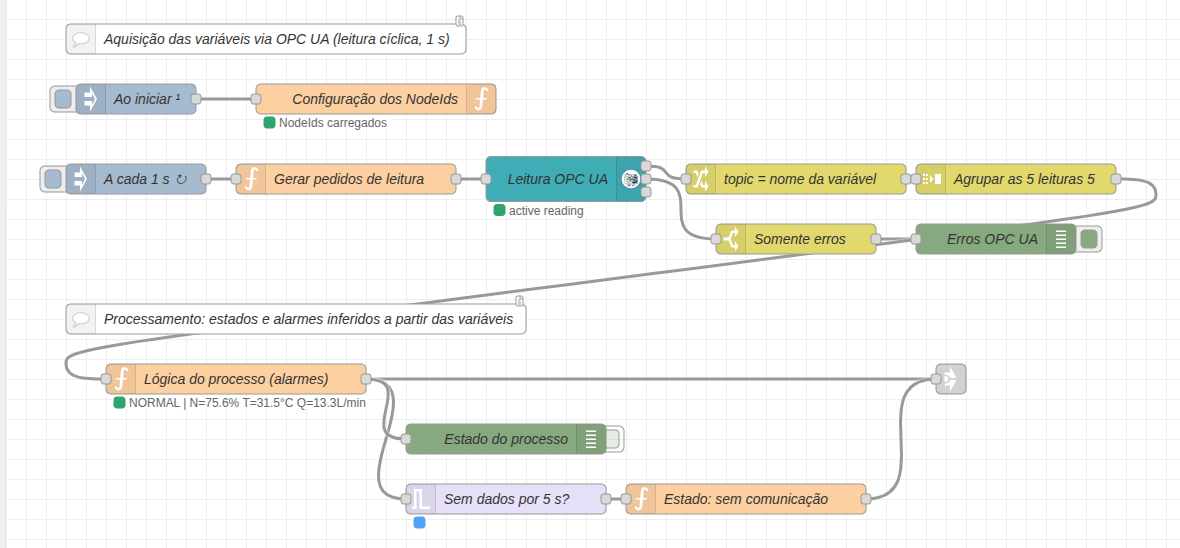
\includegraphics[width=\linewidth]{figuras/fluxo1.png}
\caption{Fluxo de aquisição OPC UA e lógica do processo.}
\label{fig:fluxo1}
\end{figure}

% ================================================================== 5
\section{Processamento no Node-RED}

O Node-RED não apenas encaminha os dados: o nó \emph{Lógica do processo}
(função JavaScript) infere estados e alarmes a partir das variáveis. A
Tabela~\ref{tab:logica} lista os critérios.

\begin{table}[H]
\centering
\small
\caption{Informações inferidas e critérios utilizados.}
\label{tab:logica}
\begin{tabularx}{\linewidth}{@{}>{\raggedright\arraybackslash}p{3.3cm} >{\raggedright\arraybackslash}p{4.6cm} L@{}}
\toprule
\textbf{Informação} & \textbf{Critério} & \textbf{Justificativa} \\
\midrule
Possível falha de bombeamento &
Bomba ligada \textbf{e} vazão $< 5$~L/min durante 3 leituras seguidas ($\approx$3~s) &
Com a bomba ligada, a vazão normal fica entre 12 e 16~L/min. Vazão muito baixa
indica sucção sem líquido, válvula fechada, entupimento ou falha do motor. A
confirmação por 3~s evita alarme falso por uma leitura isolada. \\
\addlinespace
Nível alto &
Nível $\geq$ \texttt{LimiteNivelAlto} (lido do servidor) &
Risco de transbordamento. O limite fica no servidor OPC UA e pode ser
ajustado pelo operador no \emph{dashboard}. \\
\addlinespace
Nível baixo &
Nível $\leq 20$\% &
Abaixo disso a bomba pode succionar ar e operar a seco. \\
\addlinespace
Temperatura alta &
Temperatura $> 40$~°C &
A faixa normal simulada é de 28 a 34~°C. O limite fica acima dela, com
margem, para não gerar alarmes falsos. \\
\addlinespace
Estado da planta &
\texttt{FALHA} se houver falha de bombeamento; \texttt{ALARME} se houver outro
alarme; senão \texttt{NORMAL} &
Resume a situação em uma única indicação para o operador. \\
\addlinespace
Falha de comunicação &
Nenhuma leitura completa em 5~s (nó \emph{trigger}) &
Sem comunicação os dados ficam congelados. O operador precisa saber disso
para não confiar em valores antigos. \\
\bottomrule
\end{tabularx}
\end{table}

A saída da lógica é um único objeto com o estado do processo, que alimenta o
\emph{dashboard} e a publicação MQTT. Ela inclui os valores arredondados, o
estado da bomba, o estado da planta e a lista de alarmes ativos, com código,
severidade e mensagem:

\begin{lstlisting}
{ "timestamp": "2026-11-16T21:52:46.128Z",
  "nivel": 73.4, "temperatura": 32.8, "vazao": 2.6,
  "bombaLigada": true, "limiteNivelAlto": 90,
  "estadoBomba": "LIGADA", "estadoPlanta": "FALHA", "comunicacaoOk": true,
  "alarmes": [ { "codigo": "FALHA_BOMBEAMENTO", "severidade": "falha",
                 "mensagem": "Possível falha de bombeamento: bomba ligada com
                              vazão de 2.6 L/min (mínimo 5 L/min)" } ] }
\end{lstlisting}

% ================================================================== 6
\section{Publicação MQTT}

\subsection{Estrutura de tópicos}

Os tópicos seguem a hierarquia física da planta,
\texttt{fabrica/<linha>/<equipamento>/<grandeza>}. Assim, um assinante pode
escolher o nível de detalhe com os curingas do MQTT: \texttt{fabrica/\#}
recebe tudo, \texttt{fabrica/linha01/tanque01/\#} recebe só o tanque e
\texttt{fabrica/+/+/vazao} recebe a vazão de todas as linhas e equipamentos.

\begin{table}[H]
\centering
\small
\caption{Tópicos MQTT publicados pelo Node-RED.}
\label{tab:topicos}
\begin{tabularx}{\linewidth}{@{}l l c c L@{}}
\toprule
\textbf{Tópico} & \textbf{Conteúdo} & \textbf{QoS} & \textbf{Retain} & \textbf{Quando} \\
\midrule
\texttt{fabrica/linha01/tanque01/nivel}       & número (\%)      & 0 & não & a cada 1 s \\
\texttt{fabrica/linha01/tanque01/temperatura} & número (°C)      & 0 & não & a cada 1 s \\
\texttt{fabrica/linha01/bomba01/vazao}        & número (L/min)   & 0 & não & a cada 1 s \\
\texttt{fabrica/linha01/bomba01/estado}       & LIGADA/DESLIGADA & 1 & sim & a cada 1 s \\
\texttt{fabrica/linha01/status}               & JSON consolidado & 1 & sim & a cada 1 s \\
\texttt{fabrica/linha01/alarmes}              & JSON de alarmes  & 1 & sim & na mudança \\
\texttt{fabrica/linha01/nodered/conexao}      & online/offline   & 1 & sim & conexão (LWT) \\
\bottomrule
\end{tabularx}
\end{table}

As escolhas de QoS e \emph{retain} foram as seguintes:

\begin{itemize}
  \item \textbf{Medições} usam QoS~0 e não ficam retidas: um novo valor chega
        a cada segundo, então perder uma amostra não tem impacto.
  \item \textbf{Estado, status e alarmes} usam QoS~1, que garante a entrega
        ao broker, e ficam retidos. Um cliente que se conecta depois recebe o
        último estado na hora, sem esperar o próximo evento.
  \item \textbf{Alarmes} só são publicados quando o conjunto de alarmes muda.
        O assinante recebe um evento por entrada ou saída de alarme, em vez da
        mesma mensagem a cada segundo.
  \item \textbf{Conexão do Node-RED:} o broker foi configurado com
        \emph{birth}, \emph{close} e \emph{last will} em
        \texttt{fabrica/linha01/nodered/conexao}. Se o Node-RED cair, o broker
        publica \texttt{offline} e os assinantes sabem que os dados pararam de
        chegar.
\end{itemize}

\subsection{Payload estruturado}

O tópico \texttt{fabrica/linha01/status} reúne várias informações em uma única
mensagem JSON:

\begin{lstlisting}
{ "timestamp": "2026-11-16T21:52:42.127Z",
  "tanque01": { "nivel": 76.2, "temperatura": 32.7, "limiteNivelAlto": 90 },
  "bomba01":  { "estado": "LIGADA", "vazao": 15.1 },
  "estadoPlanta": "NORMAL",
  "alarmesAtivos": [] }
\end{lstlisting}

O fluxo de publicação (aba \emph{2 -- Publicação MQTT}) está na
Figura~\ref{fig:fluxo2}. Como verificação, a aba \emph{4 -- Assinante MQTT}
(Figura~\ref{fig:fluxo4}) mostra o próprio Node-RED também como
\emph{subscriber}: ele assina \texttt{fabrica/linha01/alarmes} e
\texttt{fabrica/\#}.

\begin{figure}[H]
\centering
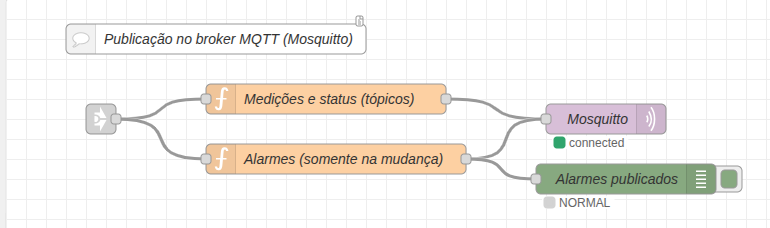
\includegraphics[width=0.62\linewidth]{figuras/fluxo2.png}
\caption{Fluxo de publicação MQTT.}
\label{fig:fluxo2}
\end{figure}

\begin{figure}[H]
\centering
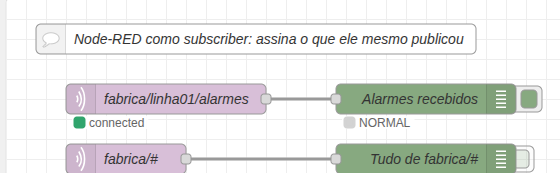
\includegraphics[width=0.5\linewidth]{figuras/fluxo4.png}
\caption{Node-RED atuando como assinante MQTT.}
\label{fig:fluxo4}
\end{figure}

\subsection{Broker e cliente adicional}

O broker Mosquitto roda em um contêiner Docker (arquivo
\texttt{docker-compose.yml}) com o arquivo de configuração
\texttt{mosquitto/config/mosquitto.conf}, que abre a porta 1883 e aceita
clientes anônimos (uso local). O cliente MQTT adicional é o
\texttt{mosquitto\_sub}:

\begin{lstlisting}[language=bash]
docker exec -it mosquitto-sda mosquitto_sub -h localhost -t "fabrica/#" -v
\end{lstlisting}

% ================================================================== 7
\section{Dashboard de supervisão}

O \emph{dashboard} foi feito com o FlowFuse Dashboard 2.0, dentro do próprio
Node-RED, e fica em \texttt{http://localhost:1880/dashboard}. Ele não usa banco
de dados: os gráficos guardam na memória os últimos 10 minutos enquanto o
fluxo está rodando. A Tabela~\ref{tab:dashboard} relaciona os requisitos do
enunciado aos elementos implementados.

\begin{table}[H]
\centering
\small
\caption{Requisitos do dashboard e elementos implementados.}
\label{tab:dashboard}
\begin{tabularx}{\linewidth}{@{}>{\raggedright\arraybackslash}p{5.2cm} L@{}}
\toprule
\textbf{Requisito} & \textbf{Implementação} \\
\midrule
Valores atuais das principais variáveis & Medidores de nível, temperatura e vazão \\
Pelo menos dois gráficos temporais & Gráficos de nível (com a linha do limite de nível alto), vazão e temperatura \\
Estado de um equipamento & Indicador LIGADA/DESLIGADA da bomba \\
Indicação visual de alarmes & Painel ``Estado da planta e alarmes'' (verde = NORMAL, laranja = ALARME, vermelho piscando = FALHA ou SEM COMUNICAÇÃO), lista de alarmes ativos e aviso \emph{pop-up} quando surge um novo alarme \\
Comandos (escrita OPC UA) & Chave para ligar/desligar a bomba (escreve \texttt{Bomba01.Ligada}, Boolean) e controle do limite de nível alto (escreve \texttt{Tanque01.LimiteNivelAlto}, Int32) \\
\bottomrule
\end{tabularx}
\end{table}

A Figura~\ref{fig:dash_normal} mostra o \emph{dashboard} em operação normal e
a Figura~\ref{fig:fluxo3}, o fluxo correspondente. Os comandos usam um segundo
nó \emph{OPC UA Client} com a ação \texttt{write}. Os nós \emph{rbe} (``só na
mudança'') atualizam a chave e o controle deslizante com o valor lido do
servidor apenas quando ele muda. Assim, uma alteração feita direto no Prosys
também aparece no \emph{dashboard}.

\begin{figure}[H]
\centering
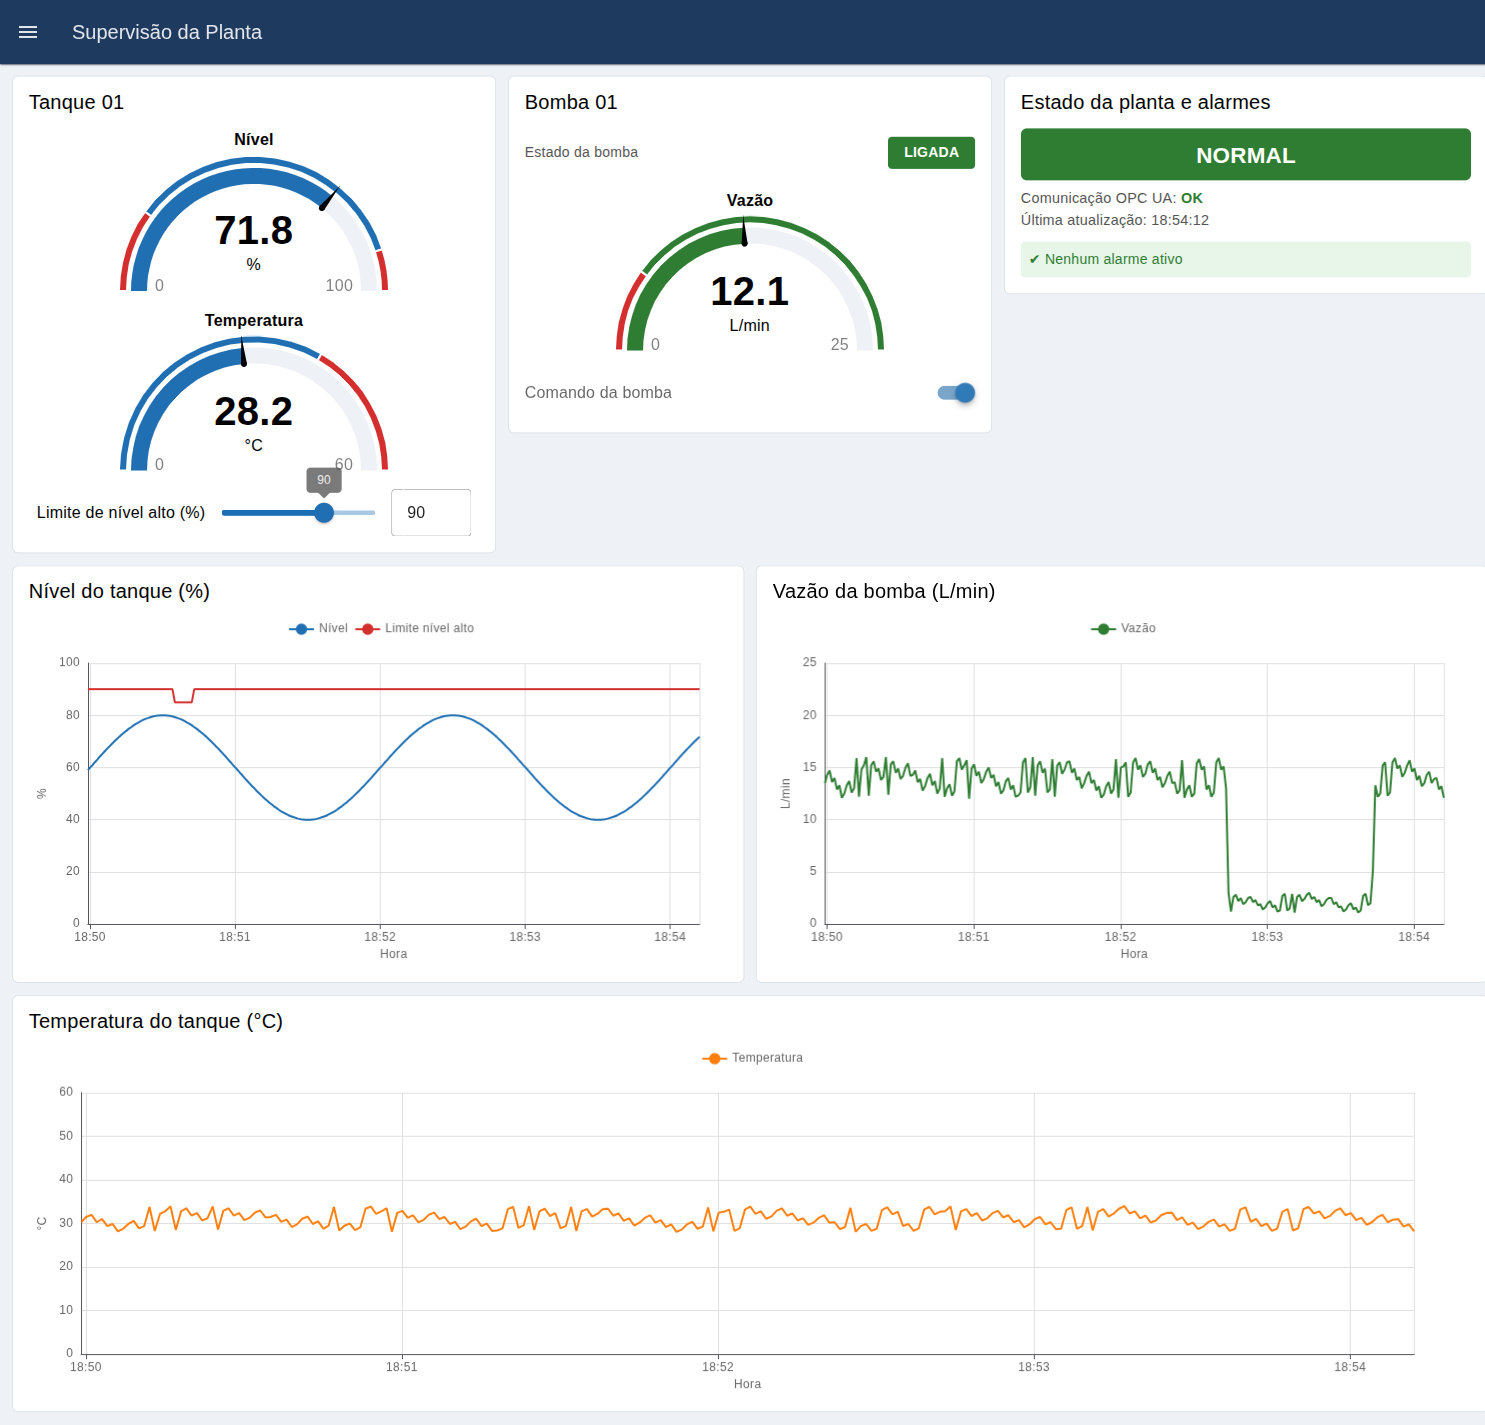
\includegraphics[width=0.92\linewidth]{figuras/dashboard_normal.png}
\caption{Dashboard em operação normal, com dados do Prosys. O histórico recente mostra a alteração do limite de nível alto feita pelo dashboard (por volta de 18:50) e a falha de bombeamento provocada seguida da recuperação (18:52--18:53).}
\label{fig:dash_normal}
\end{figure}

\begin{figure}[H]
\centering
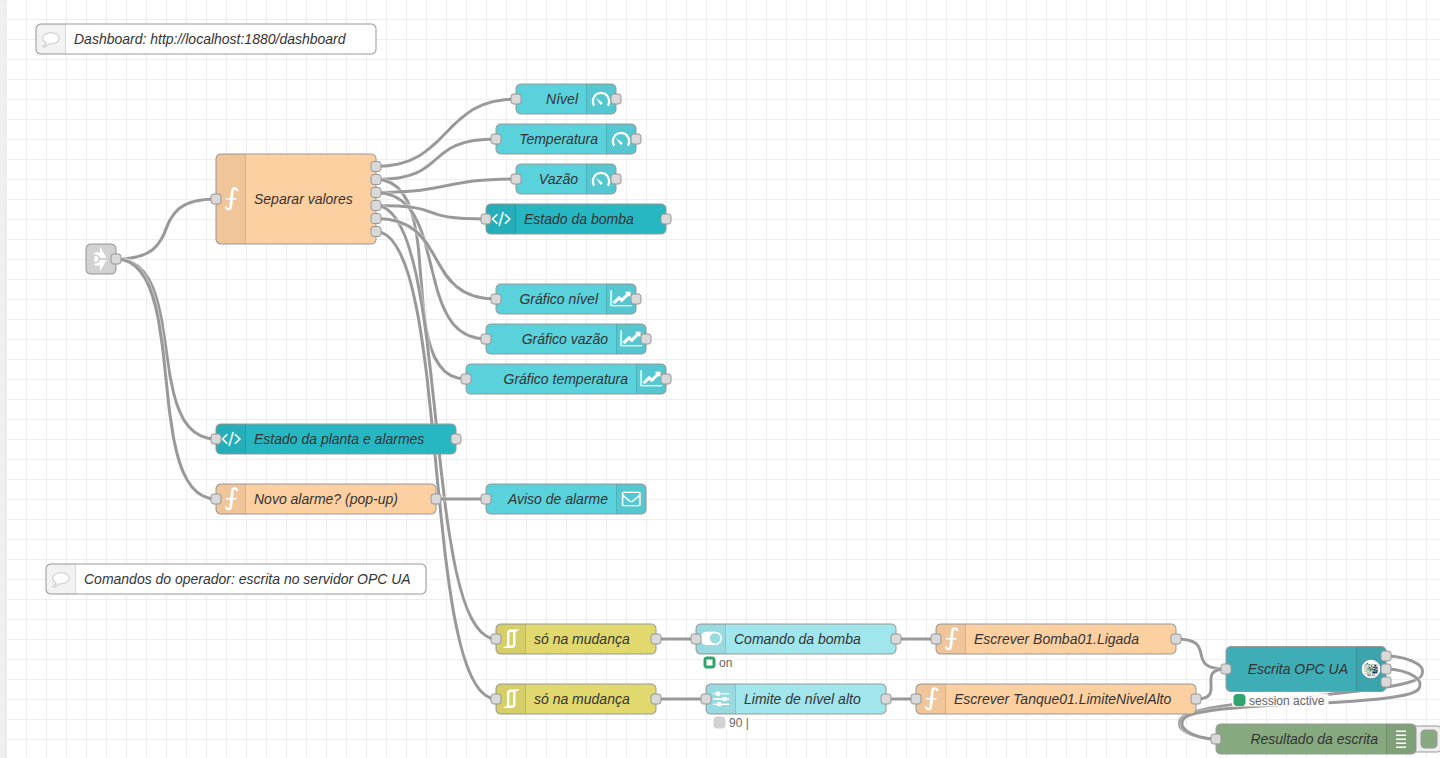
\includegraphics[width=\linewidth]{figuras/fluxo3.png}
\caption{Fluxo do dashboard e dos comandos de escrita OPC UA.}
\label{fig:fluxo3}
\end{figure}

% ================================================================== 8
\section{Demonstração de condição anormal}

A falha provocada na demonstração foi a \textbf{falha de bombeamento}: com a
bomba ligada, a simulação da variável \texttt{Vazao} foi alterada no Prosys de
12--16~L/min para valores aleatórios entre 1 e 3~L/min (campos \emph{Min Value}
e \emph{Max Value}). A
sequência pedida no enunciado foi observada da seguinte forma:

\begin{enumerate}
  \item \textbf{Aquisição via OPC UA:} a leitura cíclica passou a trazer
        vazões entre 1 e 3~L/min com \texttt{Ligada = true}.
  \item \textbf{Identificação automática:} após 3 leituras seguidas abaixo de
        5~L/min, a lógica gerou o alarme \texttt{FALHA\_BOMBEAMENTO} e mudou o
        estado da planta para \texttt{FALHA}.
  \item \textbf{Alteração do dashboard:} o painel de estado ficou vermelho e
        passou a piscar, o alarme apareceu na lista e o medidor e o gráfico de
        vazão mostraram a queda (Figura~\ref{fig:dash_falha}).
  \item \textbf{Alarme:} apareceu um aviso \emph{pop-up} com a descrição da
        falha.
  \item \textbf{Publicação MQTT:} foi publicada uma mensagem em
        \texttt{fabrica/linha01/alarmes}, e o \texttt{status} passou a conter
        \texttt{"estadoPlanta": "FALHA"}.
  \item \textbf{Recepção por um cliente MQTT:} o \texttt{mosquitto\_sub}
        recebeu as mensagens (Listagem~\ref{lst:mqtt}). As duas primeiras
        leituras baixas (3 e 1,2~L/min) ainda aparecem como \texttt{NORMAL}
        por causa da confirmação de 3~s; na terceira (2,6~L/min) o estado muda
        para \texttt{FALHA}.
\end{enumerate}

\begin{lstlisting}[caption={Mensagens recebidas pelo cliente \texttt{mosquitto\_sub} durante a falha (trecho).},label={lst:mqtt}]
fabrica/linha01/bomba01/vazao 13
fabrica/linha01/status {"timestamp":"2026-11-16T21:52:43.126Z", ... "vazao":13},"estadoPlanta":"NORMAL","alarmesAtivos":[]}
fabrica/linha01/bomba01/vazao 3
fabrica/linha01/status {"timestamp":"2026-11-16T21:52:44.127Z", ... "vazao":3},"estadoPlanta":"NORMAL","alarmesAtivos":[]}
fabrica/linha01/bomba01/vazao 1.2
fabrica/linha01/status {"timestamp":"2026-11-16T21:52:45.127Z", ... "vazao":1.2},"estadoPlanta":"NORMAL","alarmesAtivos":[]}
fabrica/linha01/bomba01/vazao 2.6
fabrica/linha01/status {"timestamp":"2026-11-16T21:52:46.128Z", ... "vazao":2.6},"estadoPlanta":"FALHA","alarmesAtivos":["FALHA_BOMBEAMENTO"]}
fabrica/linha01/alarmes {"timestamp":"2026-11-16T21:52:46.128Z","estadoPlanta":"FALHA","quantidade":1,"alarmes":[{"codigo":"FALHA_BOMBEAMENTO","severidade":"falha","mensagem":"Possível falha de bombeamento: bomba ligada com vazão de 2.6 L/min (mínimo 5 L/min)"}]}
\end{lstlisting}

\begin{figure}[H]
\centering
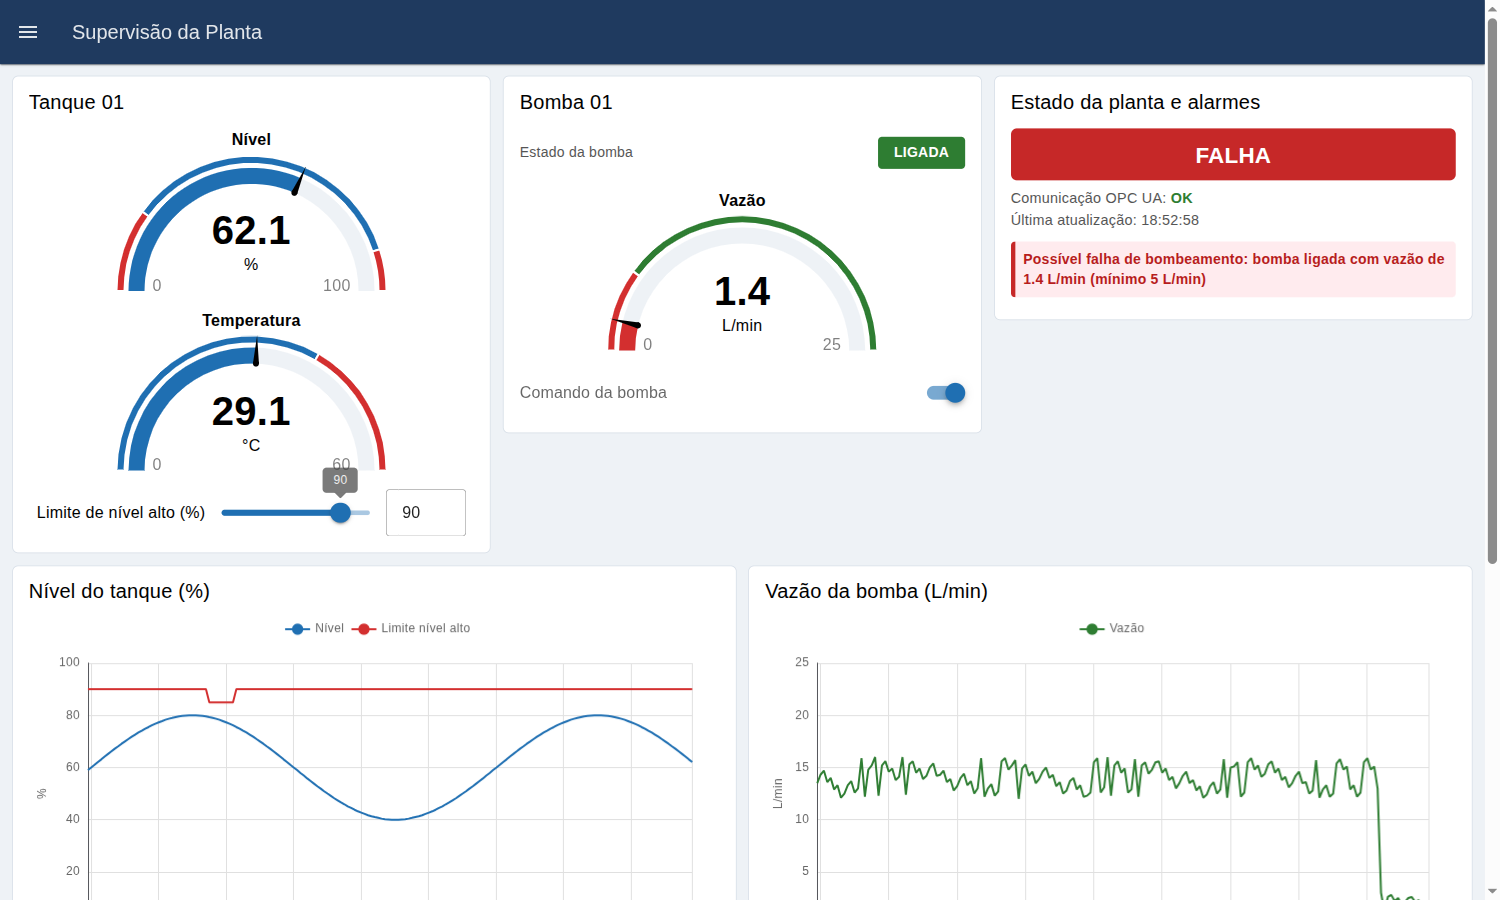
\includegraphics[width=0.92\linewidth]{figuras/dashboard_falha.png}
\caption{Dashboard durante a falha de bombeamento.}
\label{fig:dash_falha}
\end{figure}

Também foram testados os demais casos:

\begin{itemize}
  \item \textbf{Temperatura alta:} temperatura acima de 40~°C gera o estado
        \texttt{ALARME}.
  \item \textbf{Nível alto:} baixar o limite pelo \emph{dashboard} até um
        valor menor que o nível atual testa a escrita Int32.
  \item \textbf{Bomba desligada:} desligar a bomba pela chave do
        \emph{dashboard} testa a escrita Boolean e encerra o alarme de
        bombeamento, já que a vazão baixa passa a ser esperada.
  \item \textbf{Falha de comunicação:} parar o servidor OPC UA faz o estado ir
        para \texttt{SEM COMUNICAÇÃO} após 5~s. Ao reiniciar o servidor, a
        leitura volta sozinha.
\end{itemize}

% ================================================================== 9
\section{Discussão}

\paragraph{Como transportar as informações de forma organizada, interoperável e desacoplada?}
Cada tecnologia resolve uma parte do problema:

\begin{itemize}
  \item O \textbf{OPC UA} dá \emph{organização} e \emph{interoperabilidade} no
        nível do equipamento. As variáveis ficam em uma hierarquia navegável
        (objeto, pastas, variáveis), com tipo de dado, direito de acesso e
        \emph{timestamp}, e qualquer cliente OPC UA as acessa pelo endpoint e
        pelo NodeId, sem depender do fabricante.
  \item O \textbf{Node-RED} transforma \emph{dados} em \emph{informação}:
        junta as variáveis, aplica critérios do processo e produz estados e
        alarmes com significado para o operador e para outras aplicações.
  \item O \textbf{MQTT} dá o \emph{desacoplamento}. O Node-RED publica no
        broker sem saber quem vai consumir, e os assinantes não precisam saber
        quem produziu a informação nem estar conectados ao mesmo tempo (as
        mensagens retidas entregam o último estado).
\end{itemize}

\paragraph{Desacoplamento na prática.}
Durante os testes, o \texttt{mosquitto\_sub} foi aberto e fechado várias vezes
sem nenhuma alteração no fluxo que publica, e ao se conectar ele recebeu de
imediato as mensagens retidas (estado da bomba, status e alarmes). Para acrescentar uma nova aplicação, como um historiador, um painel na
nuvem ou um sistema de manutenção, basta conectá-la ao broker e assinar
\texttt{fabrica/\#} ou só os tópicos de interesse.

\paragraph{Uma aplicação, vários papéis.}
O Node-RED foi, ao mesmo tempo, \emph{cliente OPC UA} (leitura e escrita),
\emph{publisher} MQTT, \emph{subscriber} MQTT (aba 4) e interface de supervisão.
Isso mostra a flexibilidade do modelo \emph{publish/subscribe} citada no
enunciado.

\paragraph{Por que não publicar tudo direto do servidor OPC UA?}
O OPC UA usa um modelo cliente-servidor, com sessões: cada aplicação
interessada precisaria abrir uma sessão com o equipamento, o que aumenta a
carga sobre ele e o acoplamento. Com o Node-RED como ponte, o equipamento
atende um único cliente, e a distribuição para muitos consumidores fica a cargo
do broker MQTT, que foi feito para isso.

\paragraph{Limitações.}
A solução é didática: o broker aceita clientes anônimos, a conexão OPC UA não
usa criptografia e os limites de alarme estão fixos no código, exceto o de
nível alto. Em um ambiente industrial seriam necessários autenticação e TLS no
broker, certificados no OPC UA e limites configuráveis. A leitura cíclica de
1~s também poderia ser trocada por \emph{subscriptions} OPC UA (monitored
items), em que o servidor só envia as variáveis que mudam.

% ================================================================== 10
\section{Conclusão}

O trabalho implementou a arquitetura proposta de ponta a ponta: o Prosys OPC
UA Simulation Server representa o tanque e a bomba, o Node-RED adquire as
variáveis via OPC UA, infere falhas e alarmes, exibe o processo em um
\emph{dashboard} com valores atuais, gráficos, estado da bomba e alarmes, e
publica as informações em uma hierarquia de tópicos MQTT no broker Mosquitto.
Esses tópicos são recebidos por um cliente independente. A falha de
bombeamento provocada percorreu toda a cadeia, da leitura OPC UA até o cliente
MQTT, mostrando como tecnologias diferentes convivem em um sistema distribuído
de automação, cada uma no nível em que é mais adequada.

{\small\raggedright
\begin{thebibliography}{9}\setlength{\itemsep}{1pt}
\bibitem{nodered} OpenJS Foundation. \emph{Node-RED}. Disponível em: \url{https://nodered.org/}.
\bibitem{prosys} Prosys OPC. \emph{OPC UA Simulation Server}. Disponível em: \url{https://www.prosysopc.com/products/opc-ua-simulation-server/}.
\bibitem{mosquitto} Eclipse Foundation. \emph{Eclipse Mosquitto: an open source MQTT broker}. Disponível em: \url{https://mosquitto.org/}.
\bibitem{opcua} OPC Foundation. \emph{OPC Unified Architecture}. Disponível em: \url{https://opcfoundation.org/about/opc-technologies/opc-ua/}.
\bibitem{mqtt} OASIS. \emph{MQTT Version 3.1.1}. Disponível em: \url{https://docs.oasis-open.org/mqtt/mqtt/v3.1.1/mqtt-v3.1.1.html}.
\bibitem{opcuanode} \emph{node-red-contrib-opcua}. Disponível em: \url{https://flows.nodered.org/node/node-red-contrib-opcua}.
\bibitem{dashboard} FlowFuse. \emph{Node-RED Dashboard 2.0}. Disponível em: \url{https://dashboard.flowfuse.com/}.
\end{thebibliography}
}

\end{document}
